\section{重要节点检测算法在牵制控制上的研究}

第四章主要研究重要节点检测算法及算法在牵制控制上的应用。
传统重要节点检测算法在网络牵制控制中,往往效果不稳定,在不同的网络中差异巨大。
为了解决这个问题,本章对耦合强度范围这一指标进行扰动分析,衡量了单节点和多节点重要性,提出了一个网络重要节点检测算法。
该算法复杂度低,能够有效地计算出网络中的重要节点。
在六个真实网络中的实验显示,该算法容易找到被其他算法所忽视的重要节点,能够极大地增强节点对网络的控制能力。

\subsection{耦合强度范围的扰动研究}

本节分析耦合强度范围的扰动,首先从单一节点出发,选取影响能力最大的节点作为网络重要节点;同理,在多节点重要性衡量时,在误差允许的范围内,可以根据耦合强度范围的扰动情况,选取最佳的节点集合。
随后依据重要节点的检测过程,本章提出了一个贪婪算法,该算法复杂度低,能够快速计算出网络的重要节点,并给出了算法伪代码。

\subsubsection{单节点的重要性检测}

当控制网络中单个节点$ i $时,通过耦合强度范围的微分(见式子 \ref{Eq:orginperturb2} ),可以近似地计算出该节点所引起耦合强度范围的扰动:
\begin{equation}
\begin{aligned}
\Delta \omega  &= d\frac{\partial \omega}{\partial d_i}
\\
&\approx \frac{d}{\lambda_1^2}[\alpha_2R^2(X_N^i)^2-\alpha_1(X_1^i)^2]. 
\end{aligned}
\label{Eq: Delta_omega}
\end{equation}

大部分情况下,反馈强度$ d $被设置为一个固定值。因此,对于某个节点$ i $来说,定义$ PW $值:
\begin{equation}
PW(i) \approx \frac{1}{\lambda_1^2}[\alpha_2R^2(X_N^i)^2-\alpha_1(X_1^i)^2].
\label{Eq: PWi}
\end{equation}
其中,$ i $代表新增的某一控制节点,常数$ \alpha_1 $和$ \alpha_2 $与网络模型以及节点间的耦合方式有关,$ R $指的是未加控制节点$ i $前网络的传统比率判据,$ (X_1^i) $和$ (X_N^i) $代表特征向量$ X_1 $和$ X_N $的第$ i $个元素值,特征向量$ X_1 $和$ X_N $分别与控制矩阵$ C $(见式子\ref{Eq: C})的最大最小特征值$ \lambda_1 $和$ \lambda_N $对应。

节点的$ PW $值反映了该节点作为控制节点时对耦合强度范围的影响。$ PW $值越大,代表影响越大,耦合强度范围的变化更为剧烈,也就是说这个节点对耦合强度范围而言也更为重要。需要注意到的是,在大多数情况下,$ \alpha_2<<\alpha_1\approx0 $,节点的$ PW $值主要由式子$ \ref{Eq: PWi} $第一项来决定;但是在实验中发现,式子第二项对节点的$ PW $值仍有较大影响。

\subsubsection{多节点的重要性检测}

这节在单个节点对耦合强度范围的扰动的基础上,探究多个节点对耦合强度范围的影响。
当一小部分节点$ P=\{x_1,x_2,...,x_u\} (u<<N) $作为网络的牵制控制节点时,同样忽略二阶导数项,
%,在忽略了二阶导数的情况下,当一小部分节点$ P=\{x_1,x_2,...,x_u\} (u<<N) $作为网络的牵引控制节点时,
式子\ref{Eq: Lambda_eigenvector}可以改写成:
\begin{equation}
\frac{\partial\lambda_k}{\partial{d_P}} = -\sum_{i=1}^{u}(X_k^{i})^2.
\label{Eq: multiplenode}
\end{equation}
将式子\ref{Eq: multiplenode}带入耦合强度范围$ \omega $的微分中,可以得到:
\begin{equation}
\begin{aligned}
PW(P) \approx  -\frac{1}{\lambda_1^2}[\alpha_1  \sum_{i=1}^{u}{(X_1^{i})^2}-\alpha_2 R^2 \sum_{i=1}^{u}{(X_N^{i})^2}].
\end{aligned}
\label{Eq: PWP}
\end{equation}

式子 \ref{Eq: PWP} 描述了多个节点作为网络的牵制控制节点时,耦合强度范围的变化情况。同样,$ PW $值越大,代表节点集合产生的耦合强度范围扰动越大,在反馈强度$ d $不变的情况下,该节点集合所对应的耦合强度范围也就越大。
而网络的稳定状态和耦合强度范围呈正相关关系,因此该节点集合更合适当作控制节点。
在工程上,可以通过选择拥有最大$ PW $值的节点集合作为控制节点,获得尽可能大的牵制强度范围。


\subsection{算法伪代码}

本节关注于如何通过节点的$ PW $值找到最佳的控制节点集合,从而确定网络的重要节点。
总体而言,耦合强度范围的变化源于每个控制节点影响的叠加,而每个控制节点的影响可以用节点的$ PW $值来衡量。因此,可以采用贪婪算法的思想,迭代地找出局部最优节点。在每次迭代过程中,可以选择具有最大$ PW $值的节点,作为当前情况下的最佳控制节点。并在多次的迭代过程中,找到最佳控制节点集合。

算法的流程如下:

(1)给定一个网络$ G(V,E) $,节点自身的动力学方程$ f(x) $,耦合矩阵$ H $;

(2)保证李雅普诺夫指数$ L_{max} $小于0的情况下,计算$ \alpha_1 $和$ \alpha_2 $;

(3)控制节点集合$ P $的初始化,将$ P $设置为空集;

(4)得到牵制控制矩阵$ C $,并计算$ C $的最大最小特征值$ \lambda_1 $与$ \lambda_N $和与之对应的特征向量$ X_1 $与$ X_N $;

(5)计算每个节点的$ PW $值并排序,选取拥有最大$ PW $值且不属于$ P $的节点,将其作为新增的控制节点;

(6)重复步骤4-5,直到满足控制节点的个数。

算法的伪代码如下:
\floatname{algorithm}{算法}
\label{algorithm}
\renewcommand{\algorithmicrequire}{\textbf{输入:}} 
\renewcommand{\algorithmicensure}{\textbf{输出:}}
\begin{algorithm}[htp]
	\caption{基于耦合强度范围扰动的关键节点算法}
	\label{PWcode}
	\begin{algorithmic}[1]
		\REQUIRE
		原始网络$ G(V,E) $,包含$ N=|V| $个节点和$ |E| $条边;
		节点自身的动力学方程$ f(x) $;
		节点之间的耦合矩阵$ H $;
		控制节点个数$ u $。
		\ENSURE
		控制节点集合$ P $。
		\STATE 确保$ \Lambda_{max}[Df+\alpha H]<0 $的情况下,计算$ (\alpha_2, \alpha_1) $的值
		\STATE 初始化节点集合$P=\emptyset $
		\REPEAT
		\STATE 牵制控制矩阵$ C=-L-D $
		\STATE 计算牵制控制矩阵$ C $的最大最小特征值$ \lambda_1 $和$ \lambda_N $,及与之相对应的特征向量 $ X_1 $和$ X_N $
		\STATE 计算经典比率判据$ R = {\lambda_1}/{\lambda_N} $%compute classical metric ratio				
		\FOR{网络的每个节点$ i=1 $ 至 $ n $}
		\STATE  计算每个节点的$ PW $值$ PW(i) =  \frac{1}{\lambda_1^2}[\alpha_2R^2(X_1^i)^2-\alpha_1(X_N^i)^2] $
		\ENDFOR
		\STATE 选择拥有最大$ PW $值且不属于$ P $的节点$ m $
		\STATE 将点$ m $加入控制节点集合$ P $
		\UNTIL{节点集合$ P $的元素个数等于$ u $}
		\STATE 返回控制节点集合$P$
	\end{algorithmic}
\end{algorithm}

算法伪代码中,$ L $和$ D $等参数的定义已在第三章第一节稳定性分析部分给出;循环计算出新的节点后,牵制控制矩阵$ C $依然会执行$ i=1 $ 至 $ n $的循环,在实际代码过程中可以简便地用一个临时值减少循环次数。另外,不同重要节点检测算法的时间复杂度见表 \ref{table:oo} 。从表中可以看到,和其他算法相比,基于耦合强度范围扰动算法(PW方法)时间复杂度较低,较易计算出网络重要节点。

\begin{table*}[h]\centering{	
		\caption{不同算法时间复杂度比较}
		\centering
		{	\begin{tabular}{cc}
				\hline
				\hline
				算法&时间复杂度\\ \hline
				度中心性(Degree centrality)&$ O(n) $ \\
				介数中心性(Betweenness centrality)&$ O(n^3) $ \\
				接近中心性(Closeness centrality)&$ O(n^2) $ \\
				特征向量中心性(Eigenvector centrality)&$ O(n^2) $\\
				K-shell分解算法(Closeness centrality)&$ O(n^2) $\\
				PageRank&$ O(n^2) $ \\
				ESI方法&$ O(n) $ \\
				基于耦合强度范围扰动算法(PW方法)&$ O(nk) $ \\
				\hline
				\hline	
			\end{tabular}				
			\label{table:oo}
	}}
\end{table*}


\subsection{性能评估}
实验先在仿真网络上给出一个示例,说明基于耦合强度扰动方法的有效性。接下来在6个真实网络上进行了模拟实验,将提出的基于耦合强度范围扰动的算法与其他5个经典算法进行了对比分析,同时追踪观察节点的状态变化情况,从而验证了基于耦合强度范围算法的准确性。另外,实验还给不同算法得到的控制节点集合做了重叠性分析,并比较了不同算法下耦合强度范围和经典判据之间的相关关系。

\subsubsection{仿真网络上的示例}

\begin{figure}[ht]%{.5\linewidth}
	\centering
	% Requires \usepackage{graphicx}
	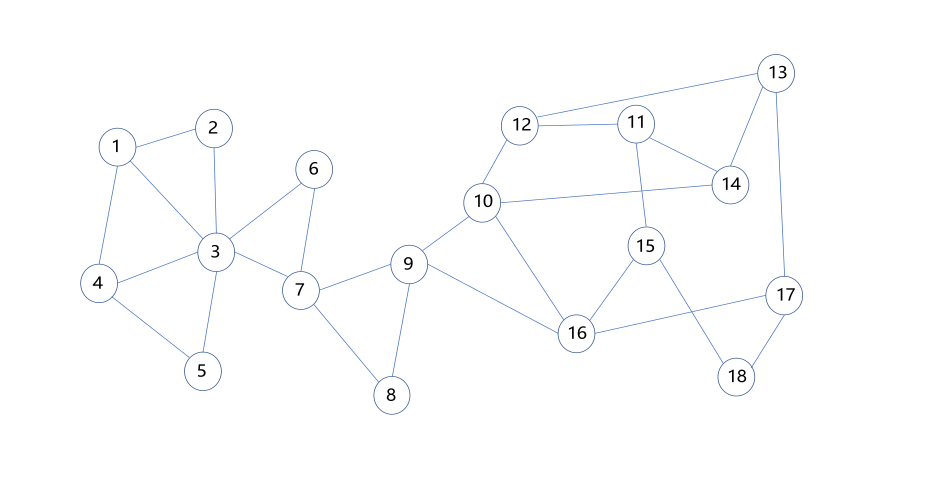
\includegraphics[width=0.8\columnwidth]{chapter4Fig/exm.png}\\
	% 
	\caption{一个仿真网络}
	\label{Fig: man-made}	
	
\end{figure}

图 \ref{Fig: man-made} 是一个仿真网络,该网络由$ 18 $个节点和$ 27 $条边构成。在这个网络上,通过不同算法计算出网络的重要节点和耦合强度范围。具体实验参数见章节 $ 4.3.3 $。

\begin{table*}[h]\centering{	
		\caption{不同算法选择的控制节点和耦合强度范围的比较}
		\centering
		\begin{tabular}{|c|c|c|}
			\hline
			算法&控制节点集合&耦合强度范围\\\hline
			\textbf{PW} 方法&(1,5,8,11,13,17)&\textbf{0.248}\\\hline
			ESI 方法&(1,2,3,4,5,7)&-2.293\\\hline
			度中心性&(1,3,7,9,10,16)&-0.098\\\hline
			介数中心性&(3,7,9,10,15,16)&0.034\\\hline
			接近中心性&(3,7,8,9,10,16)&-0.096\\\hline
			PageRank&(3,7,9,10,12,16)&0.040\\\hline	
		\end{tabular}				
		\label{table:different_al}
	}
\end{table*}

表 \ref{table:different_al} 描述了不同算法选择的控制节点集合和对应的耦合强度范围。 从表中可以明显看出,PW算法选择了控制节点集合(1,5,8,11,13,17),这组节点集合对应的耦合强度范围最大;也就是说PW算法效果更好,能够获得更大的耦合强度范围,促进节点对网络的控制作用。
其次是PageRank和介数中心性算法。这两个算法对应的耦合强度范围都大于0;也就是说,耦合强度在满足某些条件下,这些算法所对应的牵制节点能够控制整个网络。
与此相反,ESI算法、度中心性算法和最近邻算法选择的节点对应的耦合强度范围小于0;这也意味着不存在一个耦合强度,使网络达到稳定的状态。

\subsubsection{数据描述}
实验在斯坦福大学公开数据库上选取了6个真实网络,分别是:Italy powergrid, Moreno \cite{Coulomb2005}, Roundworm \cite{Duch2005}, Maayan \cite{FAA}, Facebook \cite{Viswanath2009} 和 Petster \cite{2017}。
Moreno和Roundworm分别代表的是酵母细胞中的蛋白质网络和蛔虫的蛋白质网络。蛋白质网络中,网络的节点代表蛋白质,节点之间的连边代表蛋白质之间存在某种代谢作用。Maayan则是由美国国家飞行数据中心(NFDC)采集的航空网络,该网络的节点代表机场(或服务站),连边代表NFDC所推荐的飞行路径。Facebook是社交网络,网络的节点代表Facebook用户,连边代表账户间存在相互关注关系。Petster也是社交网络,网络的节点代表在该网站上注册的宠物信息,连边代表宠物间存在朋友(或亲属)关系。

为了便于计算,在实验过程中,所有网络被调整成无向无权重网络,并且没有自环。该6个真实网络的统计信息如表\ref{table:chp4},其中,$ N $代表网络节点个数,代表网络连边数,$ H $代表网络节点的异质性,$ r $代表网络的同配性,$ <C> $网络平均聚类系数,$ <d> $代表平均最短路径长度。

\begin{table*}[h]\centering{	
		\caption{六个真实网络的结构属性特征}
			\centering
			{	\begin{tabular}{ccccccc}
					\hline
					\hline
					Network&$ N $&$ E $&$ H $&$ r $&$ <C> $&$ <d> $\\ \hline
					Italy powergrid&67&93&1.175&-0.036&0.022&6.701 \\
					Moreno&1458&1948&2.667&-0.210&0.010& 6.812\\
					Maayan&1226& 2408&1.873&-0.015&0.012&5.929 \\
					
					Facebook&744& 30023&1.633&0.503&0.559&2.558 \\
					Roundworm&453&2025&4.485&-0.226&0.098&2.664 \\
					Petster&706&10064&1.549&0.035&0.400&2.737 \\
					\hline
					\hline	
				\end{tabular}				
				\label{table:chp4}
	}}
\end{table*}

\subsubsection{对比方法与参数设置}
实验中共用选取了5种重要节点检测算法作为对比方法,分别是:度中心性(Degree centrality)、介数中心性(Betweenness centrality)、接近中心性(Closeness centrality)、PageRank算法和ESI方法。

另外,实验继续采用罗塞尔吸引子模型来模拟节点自身状态的变化情况。罗塞尔吸引子各项参数设定为:$  a_1=0.2 $, $ a_2=0.2 $,$ a_3=5 $,节点间耦合方式$ H = [1,0,0;0,0,0;0,0,0] $,则稳定点为$ \overline{\textbf{x}}=(0.008, -0.040, 0.040)^T $,$ (\alpha_2,\alpha_1)=(-4.991, -0.192) $。
在不另外声明的情况下,耦合强度$ c=0.3 $,反馈强度$ d $取网络中节点的最大度减一。动力学中方程中,节点振动频率为$ 10000 $赫兹。

\subsubsection{实验结果及分析}
首先,耦合强度取$ c=0.48 $,在Italy powergrid数据集上,不同重要节点检测算法各选取了25个节点作为牵制控制节点。在节点演化过程中,追踪了该网络上三个节点的状态变化过程,这三个节点分别是最大度节点、最小度节点和平均度节点。图 \ref{Fig: perturbation} 描述了在罗塞尔吸引子$ x_{i1} $方向上状态变化的情况。
从图中可以看到,只有在PW算法选择的控制节点下(图 \ref{Fig: perturbation} (a)),三个节点的状态在$ time>0.04 $后在$ X_{i1} $方向上是收敛的,也就是说,该网络中的节点是稳定的。对比而言,其他算法所控制的网络节点一直在震荡,无法收敛并达到稳定状态。另外,PW算法对应的耦合强度范围大于$ 0 $且最大,其他算法的耦合强度范围小于$ 0 $;所有算法对应的传统比率判据都大于$ 0 $,但PW算法的传统比率判据最大。这一方面说明PW算法效果最好,能够有效地找到牵制控制节点;另一方面也说明了耦合强度范围相较于传统判据,在描述网络牵制控制上更为有效一些。

\begin{figure}[ht]%{.5\linewidth}
	\centering
	% Requires \usepackage{graphicx}
	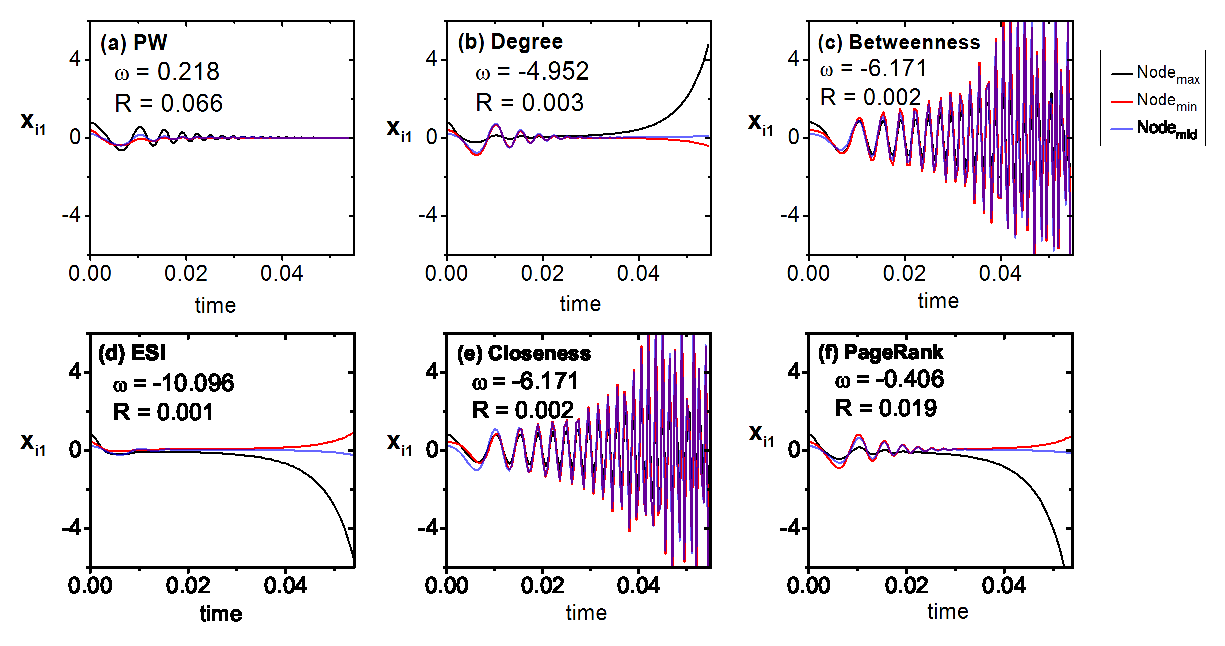
\includegraphics[width=1\columnwidth]{chapter4Fig/perturbation.eps}\\
	% 
	\caption{Italy powergrid数据集上不同方法选择节点的扰动情况}
	\label{Fig: perturbation}	
	
\end{figure}


随后,来具体观察不同网络中不同算法的实际表现情况。
图 \ref{Fig: omega} 描述了控制节点增加时耦合强度范围的变化情况。
部分情况下,随着控制节点的增加,耦合强度范围在不断扩大,网络更容易受到控制(如(a) Italy powergrid网络);同时,也存在耦合强度范围基本维持不变的情况(如(e) Roundworm网络中度中心性算法和ESI方法),因为这些算法没有选择有效的控制节点。
除此之外,在控制节点数量确定时,相较于其他启发式算法,PW算法在大部分情况下都能够获得最大的耦合强度范围。相对比而言,其他启发式算法的表现极不稳定,如在(b) Maayan网络中,牵制控制节点比例大于$ 0.2 $时,介数中心性算法和PageRank算法能获得相近的耦合强度范围,但在(d) Facebook网络中,这两种算法差异很大。由此,可以得到结论:PW算法能够稳定地得到较优的牵制控制节点集合。

\begin{figure}[htb]%{.5\linewidth}
	\centering
	% Requires \usepackage{graphicx}
	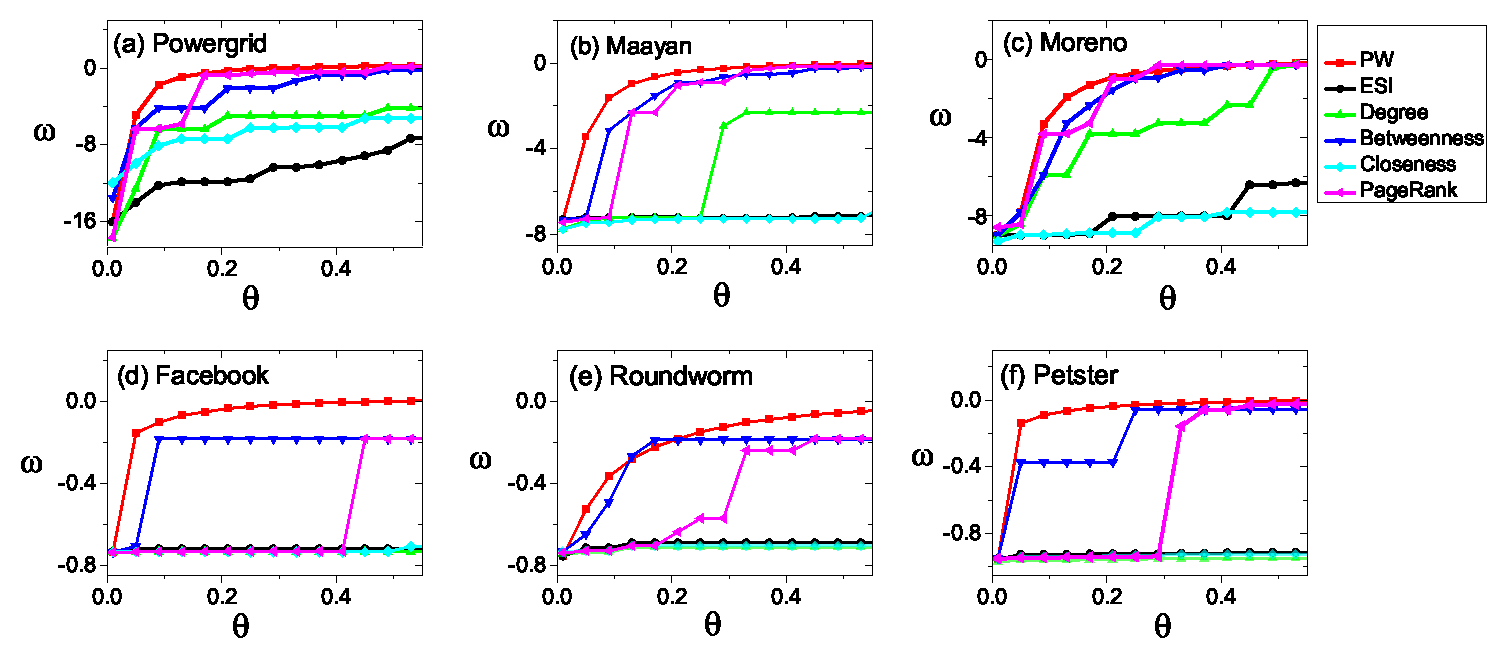
\includegraphics[width=1\columnwidth]{chapter4Fig/omega.eps}\\
	% 
	\caption{六个数据集上耦合强度范围跟随控制节点比例的变化情况}
	\label{Fig: omega}	
	
\end{figure}

同时,实验还以传统比率判据作为纵坐标,观察不同算法选择的重要节点对网络牵制控制的影响情况。图 \ref{Fig: R} 描述了不同网络在牵制控制节点比例增加时传统比率判据的变化情况。很明显,在牵制控制节点比例固定时,PW算法所对应的传统比率判据最高,也就是说,PW算法选择的牵制节点更容易控制网络。相比较而言,其他启发式算法也很不稳定,例如:在图 \ref{Fig: R} (a)中,PageRank和介数中心性算法在控制节点比例增加时,传统比率判据$ R $也在增加,也就是说,这两种算法选择的控制节点对网络的控制能力是不断增强的;但在图 \ref{Fig: R} (d)中,PageRank和介数中心性算法的比率判据的值却变化不大。由此,可以得到结论,PW算法在传统比率判据作为评判标准时,也是能够得到较优的控制节点集合的。

\begin{figure}[ht]%{.5\linewidth}
	\centering
	% Requires \usepackage{graphicx}
	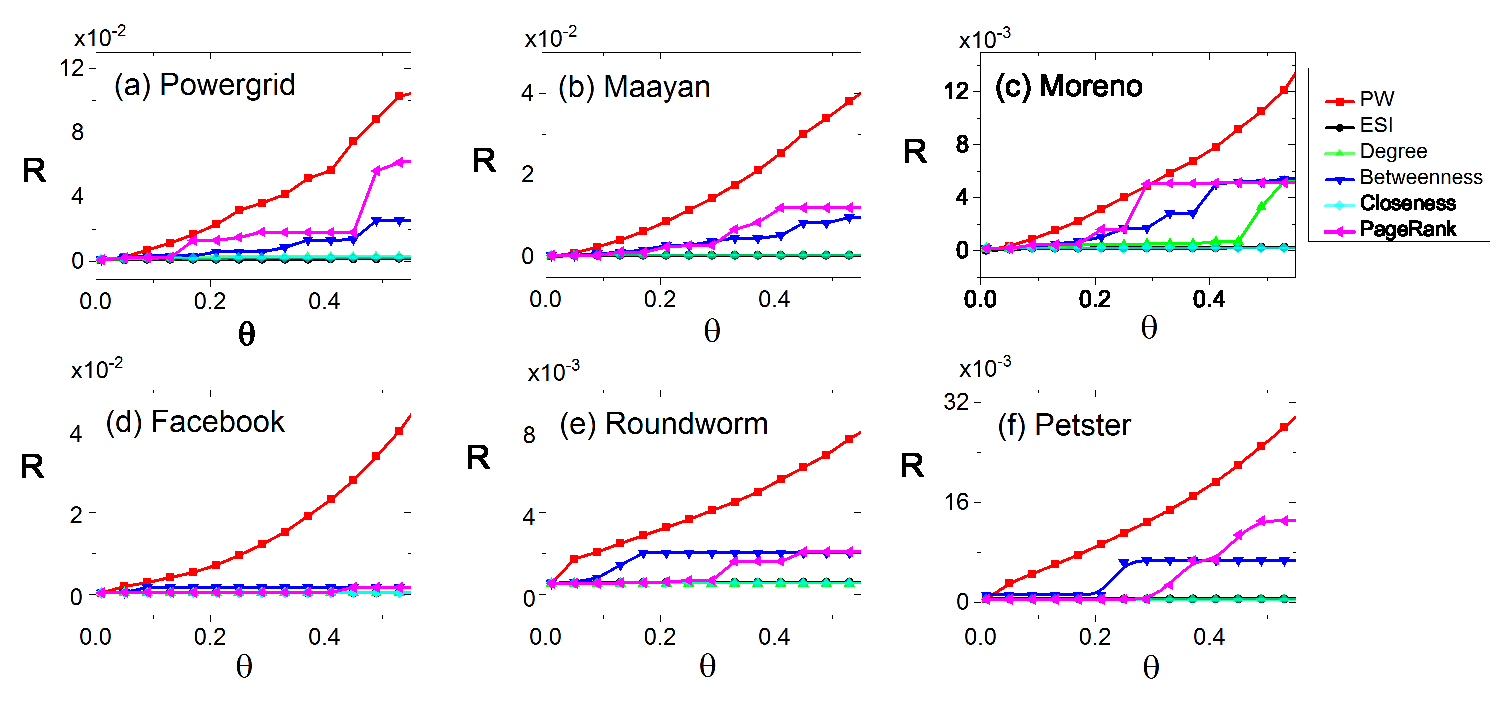
\includegraphics[width=0.9\columnwidth]{chapter4Fig/R.eps}\\
	% 
	\caption{六个数据集上传统比率判据跟随控制节点比例的变化情况}
	\label{Fig: R}	
\end{figure}

为了进一步探究$ PW $算法会选择什么样的节点作为控制节点,实验选取了30\% $ (\theta=0.3) $的节点作为控制节点,图 \ref{Fig: hdi} 描述了不同网络中PW算法和其他重要节点检测算法选择控制节点的重叠情况。从图中可以看出,六个网络中控制节点的重叠比例$ {\rm HDI}<0.3 $;也就是说,PW算法可能更倾向于选择那些容易被传统算法所忽略的节点作为控制节点。一般而言,传统方法只针对于网络或节点的某一方面特征,而且没有考虑到耦合强度范围这个指标;更重要的是,在网络控制模型中,找到最优的控制节点集合也是一个NP-hard问题。
PW算法能够快速稳定且较优地找到网络控制的重要节点,增加网络的耦合强度范围,能够很好的应用在工程中。

\begin{figure}[ht]%{.5\linewidth}
	\centering
	% Requires \usepackage{graphicx}
	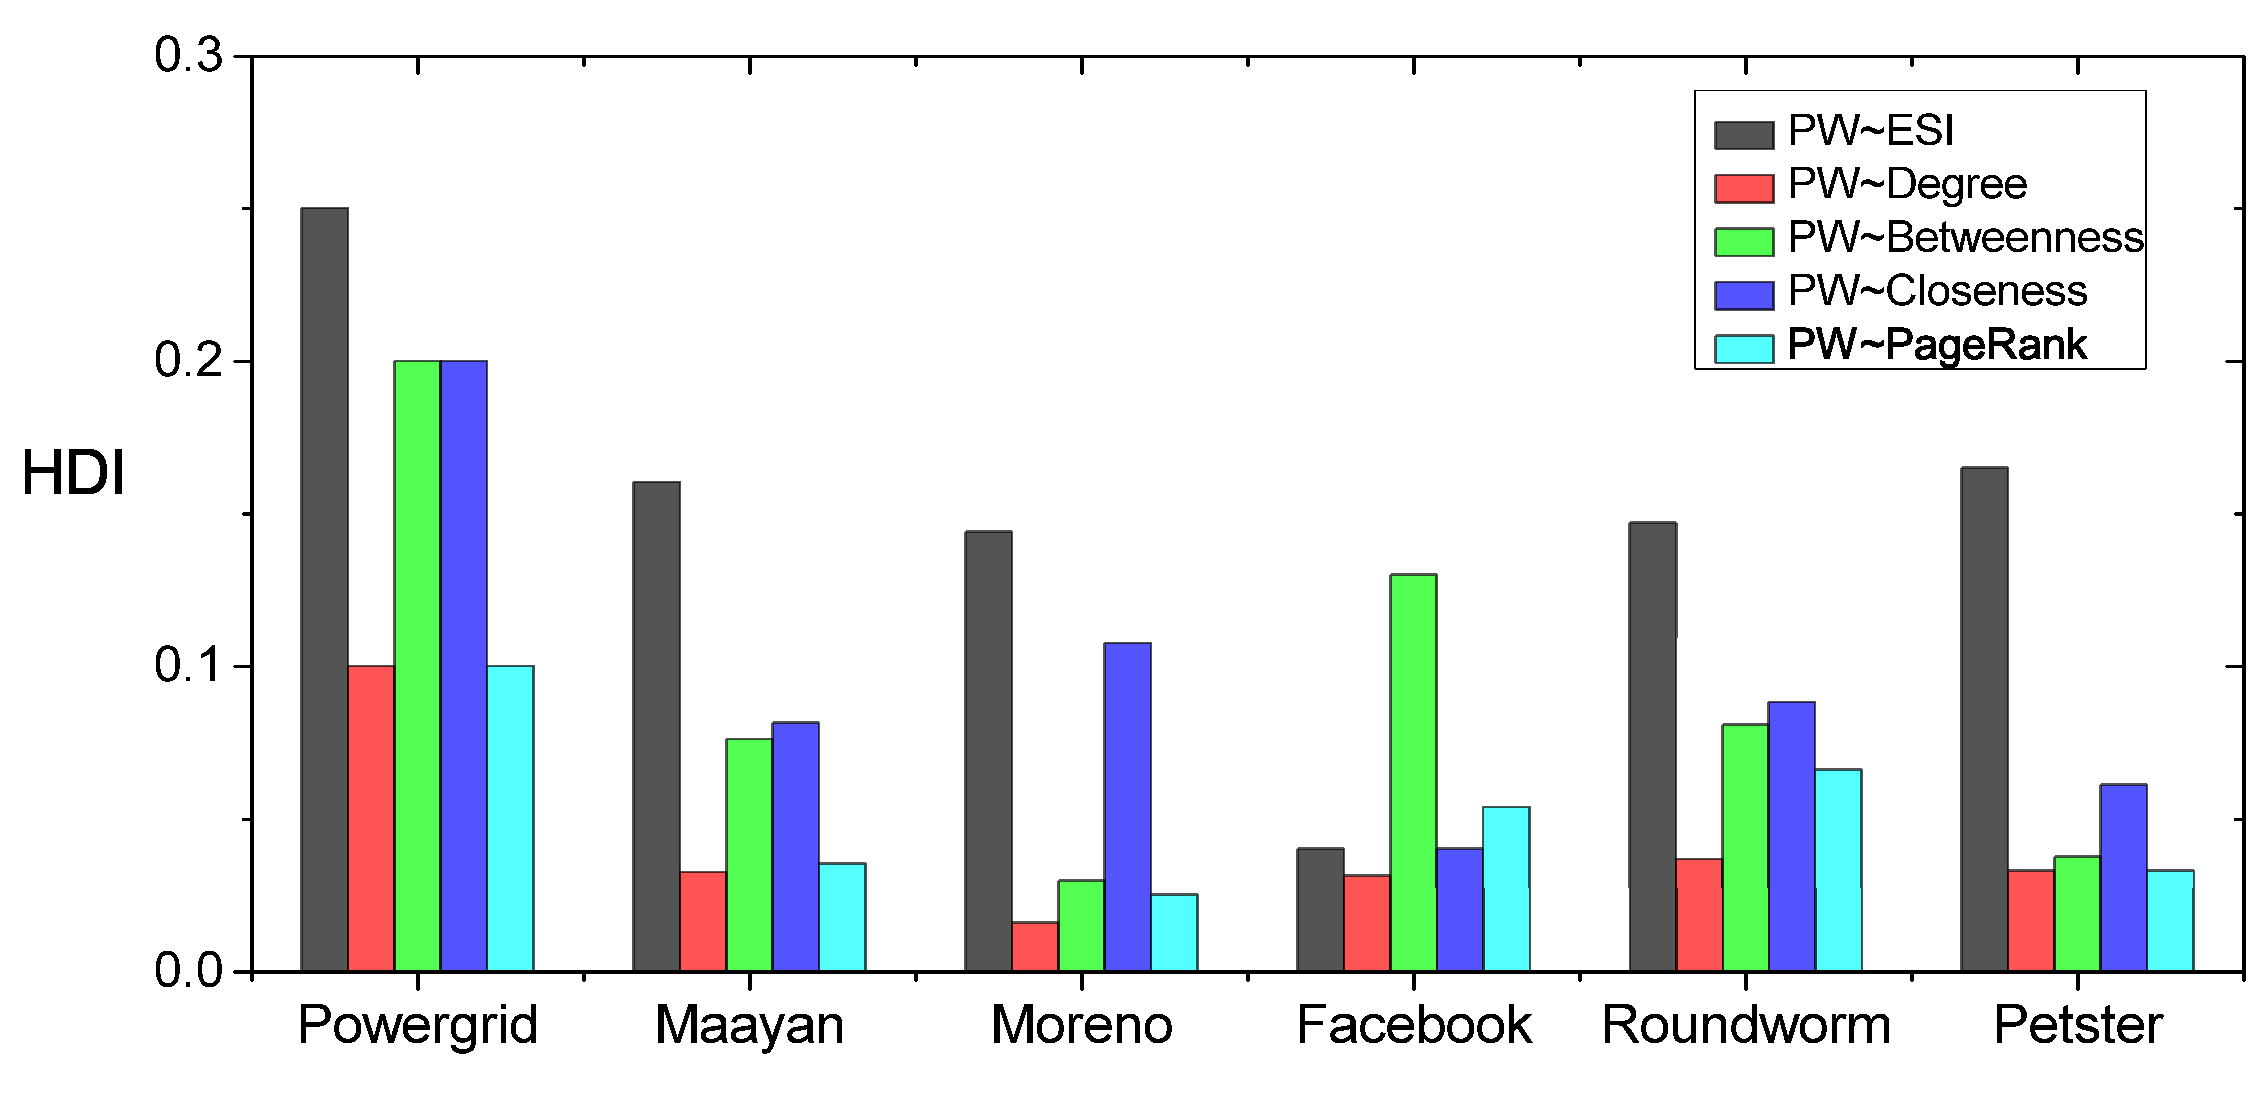
\includegraphics[width=0.9\columnwidth]{chapter4Fig/hdi.eps}\\
	% 
	\caption{六个数据集上不同方法选择节点集合的重叠情况}
	\label{Fig: hdi}	
	
\end{figure}
\begin{figure}[ht]%{.5\linewidth}
	\centering
	% Requires \usepackage{graphicx}
	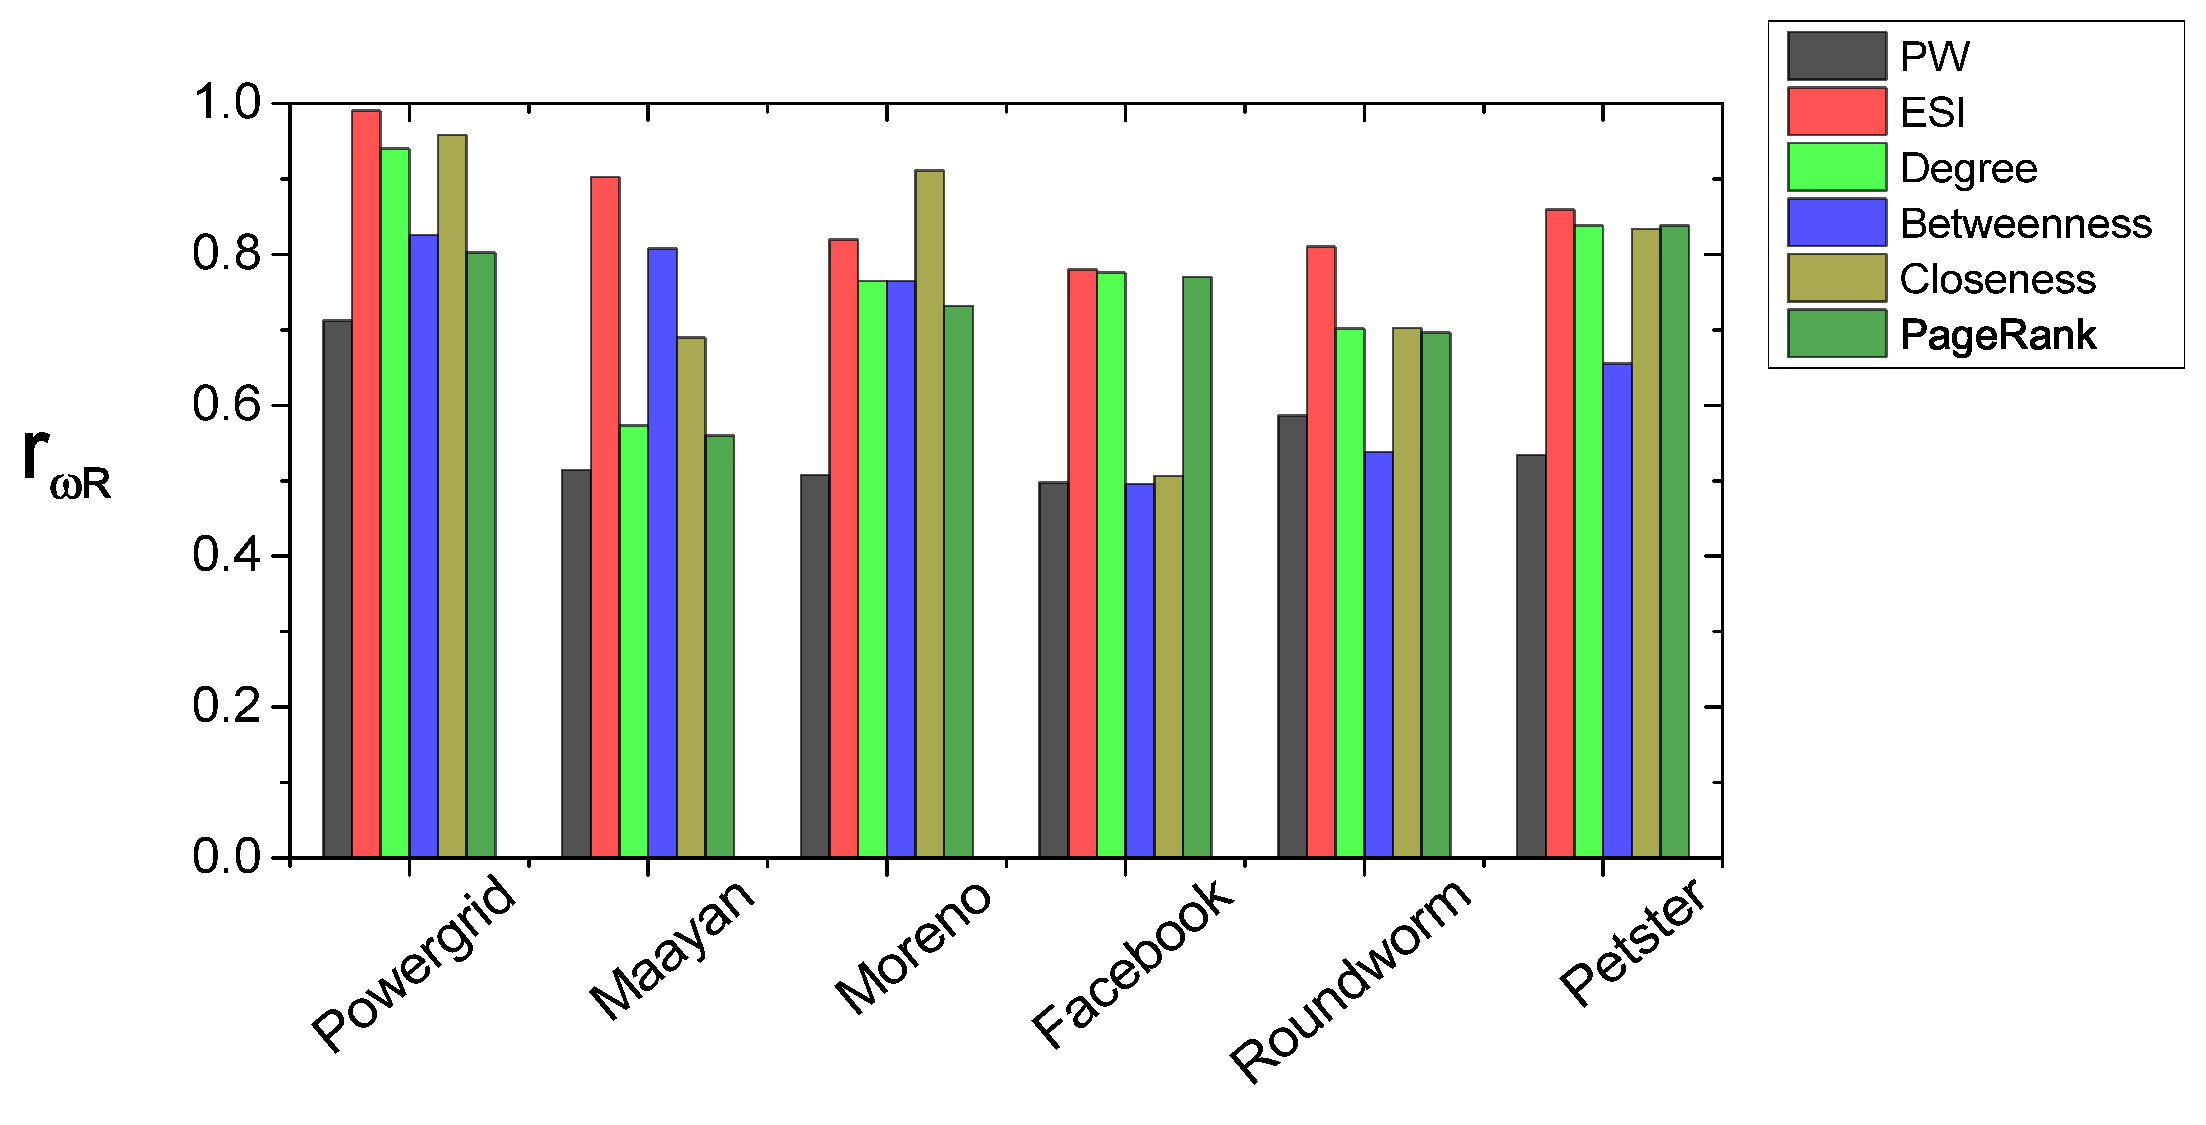
\includegraphics[width=0.9\columnwidth]{chapter4Fig/pearson.eps}\\
	% 
	\caption{六个数据集上耦合强度范围和传统比率判据的皮尔森系数}
	\label{Fig: pearson}	
	
\end{figure}

最后,实验还分析了不同网络中耦合强度范围和传统比例判据之间的相关关系。
实验在1\%至20\%的节点比例中,以1.5\%的节点作为间隔,采用不同算法选取了12组控制节点集合,计算该控制集合下传统比率判据和耦合强度范围的皮尔森系数。
图\ref{Fig: pearson}描述了这6个网络中不同算法对应的经典判据和耦合强度范围的皮尔森系数。
总体上而言,网络中皮尔森系数$ r{\omega R}>0.5 $,这代表了这两个属性之间存在强相关关系。
但对于PW算法来说,六个网络中$ r{\omega R}<0.7 $。
这是因为PW算法是局部以耦合强度范围最优的贪婪算法,而耦合强度范围最优并不能保证传统判据最优,这也说明了耦合强度范围和传统判据这两个指标之间也还是存在明显差异的。


\subsection{本章小结}
本章中,重点提出了基于耦合强度范围扰动的重要节点检测算法,并给出了其理论上的推导过程。同时,将该算法与其他经典算法做对比,验证了基于耦合强度范围扰动算法的正确性和有效性。此外,在实验中还发现该算法更倾向于选择那些被其他算法所忽视的节点,并说明了耦合强度范围和传统判据的强相关关系。

\clearpage
